\documentclass{ximera}
\input{../preamble}

\title[Dig-In:]{Area between curves}

\begin{document}
\begin{abstract}
  We find out how to compute the area of a region between two curves using the definite integral.
\end{abstract}
\maketitle


We have seen how integration can be used to find signed area between a
curve and the $x$-axis. With very little change we can find some areas
between curves. Let's see an example:


\begin{explanation}
Suppose $f>g$ on an interval $[a,b]$,

\begin{image}
\begin{tikzpicture}
	\begin{axis}[
            domain=0:3, ymax=14,xmax=3,ymin=0, xmin=0,
            axis lines =left, xlabel=$x$, ylabel=$y$,
            xtick={1,2},
            xticklabels={$a$, $b$},
            every axis y label/.style={at=(current axis.above origin),anchor=south},
            every axis x label/.style={at=(current axis.right of origin),anchor=west},
            axis on top,
          ]
          \addplot [draw=none,fill=fillp,domain=1:2] {-x^2+4*x+3} \closedcycle;
          \addplot [draw=none,fill=background,domain=1:2] {-x^3 + 7*x^2-10*x+5} \closedcycle;
          \addplot [draw=penColor,very thick] {-x^2+4*x+3};
          \addplot [draw=penColor2,very thick] {-x^3 + 7*x^2-10*x+5};
          \node at (axis cs:1,6.7) [penColor] {$f$};
          \node at (axis cs:2,4) [penColor2] {$g$};
        \end{axis}
\end{tikzpicture}
\end{image}


Above, we show the two curves together, with the desired area shaded.

It is clear from the figure that the area we want is the area under
$f(x)$ minus the area under $g(x)$, which is to say

\[
\textrm{Area} = \int_1^2 f(x)\d x-\int_1^2 g(x)\d x = \int_1^2 \left(f(x)-g(x)\right)\d x.
\]

It will also be useful to adopt the following intuitive way of thinking about this problem. In a nonrigorous way, we can think of an integral as ``summing up" an infinite number of infinitesmal quantities.  In this case, we want to find an area $A$, so we can think of \textcolor{red}{summing} up $\textcolor{blue}{\d A} = \textcolor{purple!50!blue!90!black}{(f(x) - g(x))} \textcolor{green!70!black!70!blue}{ \d x}$, where $\textcolor{green!70!black!70!blue}{ \d x}$ is the width of an infinitesmal rectangle, and $\textcolor{purple!50!blue!90!black}{(f(x) - g(x))}$ is its height.

\begin{image}
\begin{tikzpicture}
	\begin{axis}[
            domain=0:3, ymax=14,xmax=3,ymin=0, xmin=0,
            axis lines =left, xlabel=$x$, ylabel=$y$,
            xtick={1,2},
            xticklabels={$a$, $b$},
            every axis y label/.style={at=(current axis.above origin),anchor=south},
            every axis x label/.style={at=(current axis.right of origin),anchor=west},
            axis on top,
          ]
          \addplot [draw=none,fill=fillp,domain=1:2] {-x^2+4*x+3} \closedcycle;
          \addplot [draw=none,fill=background,domain=1:2] {-x^3 + 7*x^2-10*x+5} \closedcycle;
          \addplot [draw=penColor,very thick] {-x^2+4*x+3};
          \addplot [draw=penColor2,very thick] {-x^3 + 7*x^2-10*x+5};
          \node at (axis cs:1,6.7) [penColor] {$f$};
          \node at (axis cs:2,4) [penColor2] {$g$};
          \addplot [textColor, fill = blue] plot coordinates {(1.5,2.375) (1.6,2.375) (1.6, 6.84) (1.5,6.84) (1.5, 2.375)};
\addplot [color= purple!50!blue!90!black] plot coordinates {(1.6,2.375) (1.6, 6.84)};
        \end{axis}
\end{tikzpicture}
\end{image}


 \begin{image}
  \begin{tikzpicture}[scale=2,every node/.style={transform shape}]
      \draw[background, fill=background] (0,-0.5) rectangle (3.5,2.5);

      \draw[textColor, fill=blue] (1.5,0) rectangle (2,3);
    
      \node at (3,1.5) {$\color{purple!50!blue!90!black} f(x) - g(x) $};

      \node at (1.75,-0.25) {$\color{green!70!black!70!blue}{\d x} $};
    \end{tikzpicture}
  \end{image}


\begin{image}
  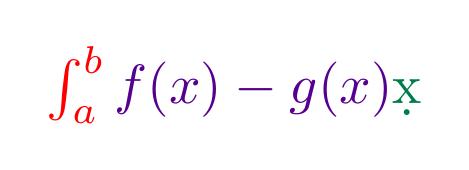
\begin{tikzpicture}[scale=2,every node/.style={transform shape}]
    \node at (0,0) {
      $\color{red} \int_{a}^{b}\color{purple!50!blue!90!black}{f(x) - g(x)} \color{green!70!black!70!blue}{\d x}\color{black}$
      };
  \end{tikzpicture}
\end{image}

We think of the integral as $\textcolor{red}{summing}$ the areas of infinitely many rectangles with infinitesmal area.  This way of thinking about integrals will be very useful to us in later, more complex, applications.

\end{explanation}

\begin{example}
If  $f(x)= -x^2+4x+3$ and 
$g(x)=-x^3+7x^2-10x+5$, and we wanted to find the area between them over the interval $1 \le x \le 2$, then we can compute

\[ 
\int_1^2 f(x)-g(x)\d x = \answer[given]{\frac{49}{12}} 
\]
\begin{hint}

\[
\int_1^2 -x^2+4x+3-(-x^3+7x^2-10x+5) \d x
\]

\begin{align*}
  &=\int_1^2 x^3-8x^2+14x-2 \d x \\
  &=\eval{\frac{x^4}{4}-\frac{8x^3}{3}+7x^2-2x}_1^2 \\
  &= \frac{16}{4} - \frac{64}{3}+28-4-(\frac{1}{4}- \frac{8}{3}+7-2) \\
  &=23-\frac{56}{3}-\frac{1}{4}\\
  &=\frac{49}{12}
\end{align*}
\end{hint}



\end{example}


In our first example, one curve was higher than the other over the
entire interval. This does not always happen.

\begin{example} Find the area between $f(x)= -x^2+4x$ and
$g(x)=x^2-6x+5$ over the interval $0 \le x \le 1$.


\begin{image}
\begin{tikzpicture}
	\begin{axis}[
            domain=-1:2, ymax=6,xmax=1.5,ymin=-0.3, xmin=-.5,
            axis lines =center, xlabel=$x$, ylabel=$y$,
	   xtick={0.5635,1},
            xticklabels={$a$,$1$}, 
            every axis y label/.style={at=(current axis.above origin),anchor=south},
            every axis x label/.style={at=(current axis.right of origin),anchor=west},
            axis on top,
          ]
          \addplot [draw=none,fill=fillp,domain=0:0.56] {x^2-6*x+5} \closedcycle;
          \addplot [draw=none,fill=background,domain=0:0.56] {-x^2+4*x} \closedcycle;
          \addplot [draw=none,fill=fillp,domain=0.56:1] {-x^2+4*x} \closedcycle;
          \addplot [draw=none,fill=background,domain=0.56:1] {x^2-6*x+5} \closedcycle;
          \addplot [draw=penColor,very thick] {-x^2+4*x};
          \addplot [draw=penColor2,very thick] {x^2 - 6*x+5};
          \node at (axis cs:1.25,3.1) [penColor] {$f$};
          \node at (axis cs:.25,4.3) [penColor2] {$g$};
          \addplot [textColor,dashed] plot coordinates {(0.5635,0) (0.5635,1.9364)};

        \end{axis}
\end{tikzpicture}
\end{image}


\begin{explanation}
 Generally we should interpret ``area'' in the usual sense, as a necessarily
positive quantity. Since the two curves cross, we need to compute two
areas and add them. First we find the intersection point of the
curves:

Letting $a$ be the x-coordinate of the point of intersection, we have $a = \answer{\frac{5-\sqrt{15}}{2}}$

\begin{hint}
\begin{align*}
  -a^2+4a &= a^2-6a+5 \\
  0 &= 2a^2-10a+5 \\
  a &= \frac{10 \pm \sqrt{100-40}}{4}\\
 a &= \frac{5 \pm \sqrt{15}}{2}.
\end{align*}

Of the two solutions, only $\frac{5-\sqrt{15}}{2}$ is within the region of intererst.
\end{hint}

Then the total area is 

\[
\textrm{Area} = \int_0^a g(x) - f(x) \d x + \int_a^1 f(x) - g(x) \d x
\]

since $g$ is above $f$ on the interval [0,a], and $f$ is above $g$ on the interval $[a,1]$.

Computing this area we have,

\[
	\textrm{Area} = \answer{5\sqrt{15} - \frac{52}{3}}
\]

\begin{hint}

\begin{align*}
\int_0^a &g(x) - f(x) \d x + \int_a^1 f(x) - g(x) \d x \\ 
 &= \int_0^a x^2-6x+5-(-x^2+4x)\d x +\int_a^1 -x^2+4x-(x^2-6x+5)\d x
\end{align*}
\begin{align*}
  &=\int_0^a 2x^2-10x+5\d x+\int_a^1 -2x^2+10x-5\d x \\
  &= \eval{\frac{2x^3}{3}-5x^2+5x}_0^a + \eval{ \frac{-2x^3}{3}+5x^2-5x}_a^1 \\
  &=5\sqrt{15}-\frac{52}{3}
\end{align*}
	
\end{hint}


\end{explanation}

\end{example}

In both of our examples above, we gave you the limits of integration
by bounding the $x$-values between $0$ and $1$. However, in some problems
you will have to do more work to determine these bounds.

\begin{example}
Find the area between $f(x)= -x^2+4x$ and
$g(x)=x^2-6x+5$.


\begin{image}
\begin{tikzpicture}
	\begin{axis}[
            domain=0:5, ymax=5,xmax=5,ymin=-5, xmin=0,
            axis lines =center, xlabel=$x$, ylabel=$y$,
 	   xtick={0.5635},
            xticklabels={$a$}, 
            every axis y label/.style={at=(current axis.above origin),anchor=south},
            every axis x label/.style={at=(current axis.right of origin),anchor=west},
            axis on top,
          ]
          \addplot [draw=none,fill=fillp,domain=.56:4] {-x^2+4*x} \closedcycle;
          \addplot [draw=none,fill=fillp,domain=.56:4.44] {x^2-6*x+5} \closedcycle;
          \addplot [draw=none,fill=background,domain=4:5] {-x^2+4*x} \closedcycle;
          \addplot [draw=none,fill=background,domain=0:1] {x^2-6*x+5} \closedcycle;
          %\addplot [draw=none,fill=fillp,domain=.56:4] {-x^2+4*x} \closedcycle;       
          \addplot [draw=penColor,very thick,smooth] {-x^2+4*x};
          \addplot [draw=penColor2,very thick,smooth] {x^2-6*x+5};
          
          \node at (axis cs:2,4.4) [penColor] {$f$};
          \node at (axis cs:1,-1) [penColor2] {$g$};
	 \node at (axis cs:4.43649,0.3) [textColor] {b};
	 \addplot [textColor,dashed] plot coordinates {(0.5635,0) (0.5635,1.9364)};
          \addplot [textColor,dashed] plot coordinates {(4.43649,0) (4.43649,-1.9364)};
        \end{axis}
\end{tikzpicture}
\end{image}

\begin{explanation}
Here we are not given a specific interval, so it must be the case that
there is a ``natural'' region involved. Since the curves are both
parabolas, the only reasonable interpretation is the region between
the two intersection points, which we found in the previous example to be 
$a=(5-\sqrt{15})/2$ and $b=(5+\sqrt{15})/2$.


Since $f \geq g$ on $[a,b]$, the total area is 

\[
\int_a^b f(x) - g(x) \d x = \answer{4\sqrt{15}}
\]


\begin{hint}
\begin{align*}
  \int_a^b -x^2+4x-(x^2-6x+5)\d x
  &=\int_a^b -2x^2+10x-5\d x \\
  &=\eval{-\frac{2x^3}{3}+5x^2-5x}_a^b \\
  &=5\sqrt{15},
\end{align*}
\end{hint}

\end{explanation}
\end{example}


\begin{example}
	Consider the region bounded by the function $f(x) = \sqrt{x-1}$, $g(x) = x-3$, and the horizontal axis.
\begin{image}

\begin{tikzpicture}
	\begin{axis}[
            domain=0:5.5, ymax=2.5,xmax=5.5, ymin=0, xmin=0,
            axis lines =center, xlabel=$x$, ylabel=$y$,
            every axis y label/.style={at=(current axis.above origin),anchor=south},
            every axis x label/.style={at=(current axis.right of origin),anchor=west},
            axis on top,
          ]
          \addplot [ fill = fillp, smooth, samples=100, domain=(0:2)] ({1+x^2},{x}) \closedcycle;
          \addplot [draw=none,fill=background,domain=0:5.2] {x-3} \closedcycle;   
          \addplot [very thick, penColor, smooth, samples=100, domain=(0:3)] ({1+x^2},{x});
          \addplot [draw=penColor2,very thick,smooth] {x-3};
          
          \node at (axis cs:2,1.3) [penColor] {$f$};
          \node at (axis cs:4,0.7) [penColor2] {$g$};


        \end{axis}
\end{tikzpicture}
\end{image}

While we could find the area of this region by breaking the computation up into the two regions $[1,3]$ and $[3,5]$ (check that $5$ is the intersection point!), there is another approach.  We can think of splitting the region up into \textbf{horizontal} rectangles.  

We can rewrite $y = \sqrt{x-1}$ as $x = y^2+1$, and we can rewrite $y = x-3$ as $x = y+3$, so we have the following picture:
s
\begin{image}
\begin{tikzpicture}
	\begin{axis}[
            domain=0:5.5, ymax=2.5,xmax=5.5, ymin=0, xmin=0,
            axis lines =center, xlabel=$x$, ylabel=$y$,
            every axis y label/.style={at=(current axis.above origin),anchor=south},
            every axis x label/.style={at=(current axis.right of origin),anchor=west},
            axis on top,
          ]
          \addplot [ fill = fillp, smooth, samples=100, domain=(0:2)] ({1+x^2},{x}) \closedcycle;
          \addplot [draw=none,fill=background,domain=0:5.2] {x-3} \closedcycle;   
          \addplot [very thick, penColor, smooth, samples=100, domain=(0:3)] ({1+x^2},{x});
          \addplot [draw=penColor2,very thick,smooth] {x-3};
          
          \node at (axis cs:2,1.3) [penColor] {$f$};
          \node at (axis cs:4,0.7) [penColor2] {$g$};

	 \addplot [textColor, fill = blue] plot coordinates {(2,1) (2,1.1) (4, 1.1) (4,1) (2, 1)};
        \end{axis}
\end{tikzpicture}
\end{image}
 
 \begin{image}
  \begin{tikzpicture}[scale=2,every node/.style={transform shape}]
      \draw[background, fill=background] (0,-0.5) rectangle (3.5,2.5);

      \draw[textColor, fill=blue] (0,0) rectangle (4,0.5);
    
      \node at (2,1) {$\color{purple!50!blue!90!black} (y+3) - (y^2+1)$};

      \node at (4.3,0.25) {$\color{green!70!black!70!blue}{\d y} $};
    \end{tikzpicture}
  \end{image}





We can think of the area of the region as the \textcolor{red}{sum} of the \textcolor{blue}{areas} of these infinitesmal rectangles from $\textcolor{red}{y=0}$ to $\textcolor{red}{y=2}$

Thus we have that the area is 

\begin{image}
  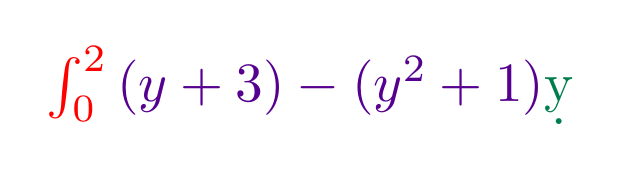
\begin{tikzpicture}[scale=2,every node/.style={transform shape}]
    \node at (0,0) {
      $\color{red} \int_{0}^{2}\color{purple!50!blue!90!black}{(y+3) - (y^2+1)} \color{green!70!black!70!blue}{\d y}\color{black}$
      };
  \end{tikzpicture}
\end{image}

Computing this we have that the area of this region is

\[
\textrm{Area} = \answer{\frac{10}{3}}
\]


\begin{hint}
\begin{align*}
	\int_0^2 (y+3) - (y^2+1) \d y &= \int_0^2 -y^2+y+2 \d y\\
	&=\eval{-\frac{y^3}{3} + \frac{y^2}{2}+2y}_0^2\\
	&=\frac{10}{3}
\end{align*}
\end{hint}
	
\end{example}


\end{document}
